\documentclass{article}
\usepackage{graphicx}
\usepackage{fancyvrb}

\begin{document}

\section{Coding}
You can try your main loop without scheduling events by setting the \verb+schedulingFlag+ to false.

\hskip-1cm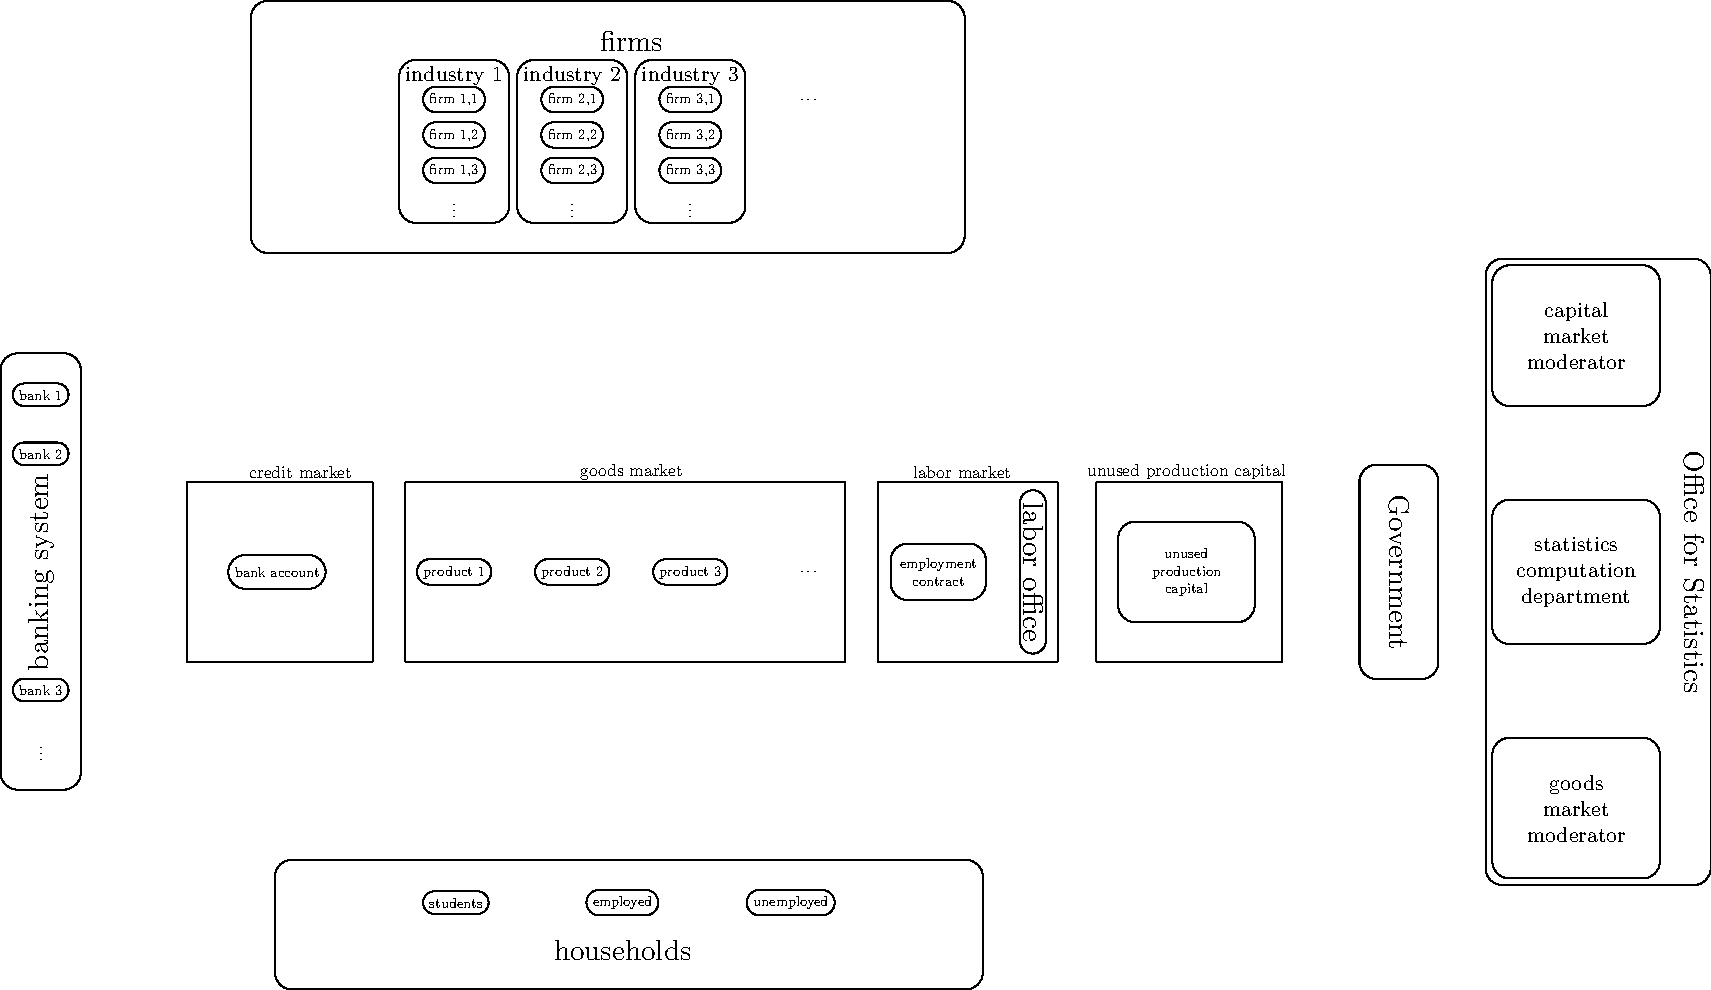
\includegraphics[scale=0.5]{agents_and_interactions_figure1.pdf}

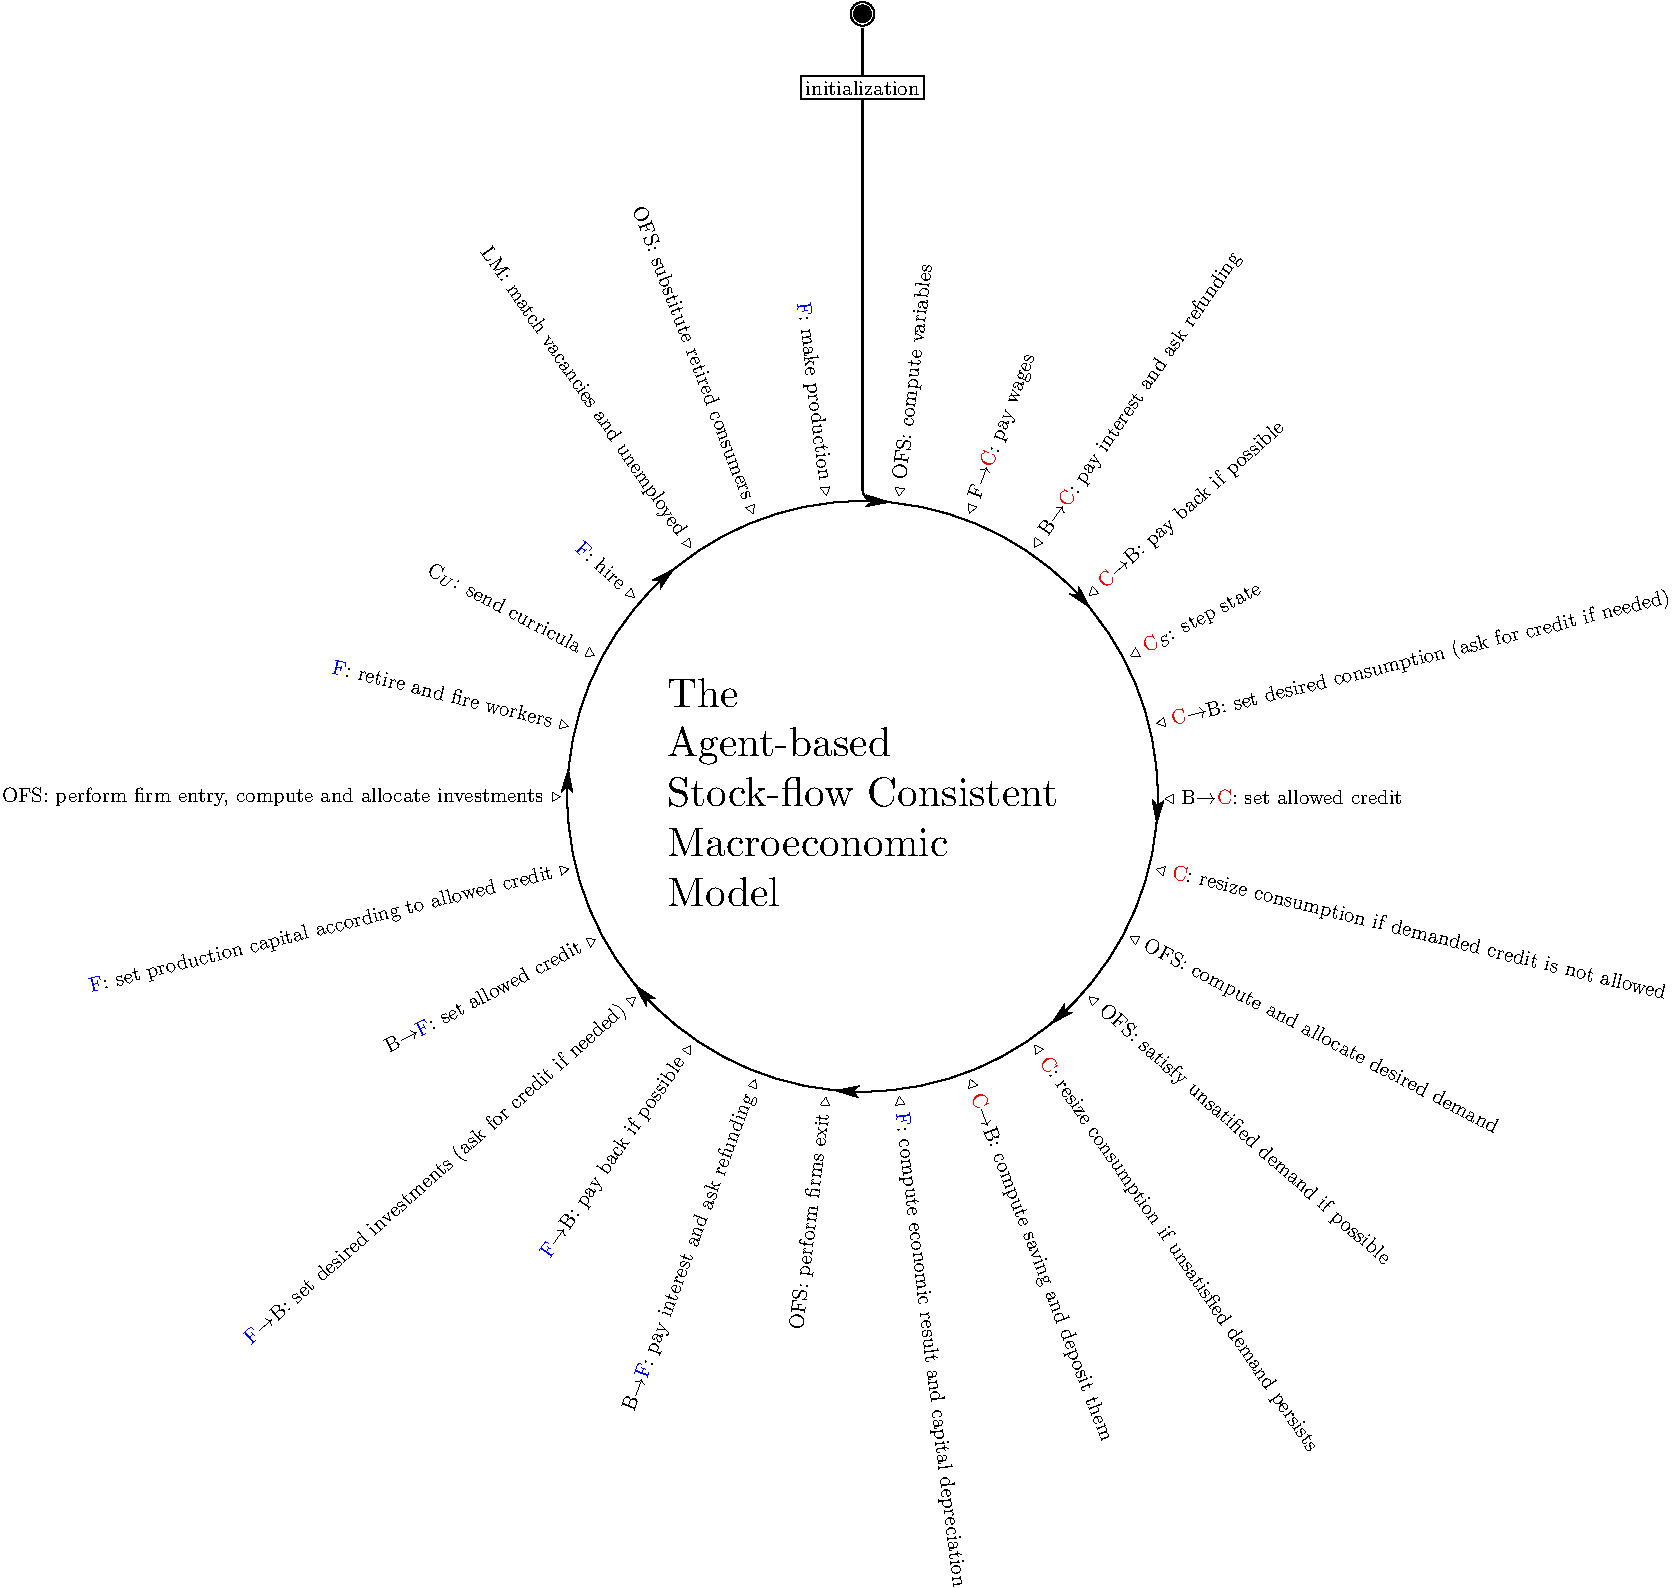
\includegraphics[scale=0.5]{visual.pdf}
\section{Bank-Consumer relationship}
Each consumer is endowed with a bank account. The bank-consumer relationship progresses by the following steps:

\begin{enumerate}
	\item banks account interests and ask for loan repayments to indebted consumers
	\item consumers refund if possible (if they have enough financial resources)
	\item the software performs a technical step by resetting some variables of the bank accounts (\dots)
	\item consumers asks for new credit
	\item banks decide how much credit to allow
	\item consumers adjust desired consumption according to allowed credit. 
		
		Then, consumers try to gather the desired level of goods on the market. The effective level of consumption is established: it may be less or equal to the desired consumption.
	\item consumers adjust their bank accounts (deposits and loans) according to effective consumption.
\end{enumerate}

%In the following we will present the dynamics of these events in some cases.
Let's consider the consumer-bank dynamics in some specific cases.

\subsection{Indebted Consumers}
%\subsubsection*{Step 1: interests and ask for repayments}
\subsubsection*{Step 1: interests and loans repayment}

Consumers can be customers of several banks.

First of all, the banks account the interest rate.

Suppose that after accounting interest rate, we have the following situation
\begin{verbatim}
bank 1 account =   10
bank 2 account = -150
bank 3 account =  -50
\end{verbatim}

The bank assumes that indebted consumers (those with a negative bank account) ask for the whole renewal of the debt:

\begin{verbatim}
bank 1 account =   10  demanded credit =    0
bank 2 account = -150  demanded credit = -150
bank 3 account =  -50  demanded credit =  -50
\end{verbatim}

Each bank with a negative account can ask for refunding. In this case the allowed credit is lower (in absolute value) than the demanded credit.
Suppose bank account 2 and 3 are as follows:

\begin{verbatim}
bank 1 account =   10  demanded credit =    0 allowed credit =    0
bank 2 account = -150  demanded credit = -150 allowed credit = -130 
bank 3 account =  -50  demanded credit =  -50 allowed credit =  -45
\end{verbatim}

In this example, the consumer needs 25 to satisfy banks' request.

\subsubsection*{step 2: refunding}
The consumer refunds her bank account if she has enough income (to refund) and, in any case, refunds an amount that allows a subsistence consumption level. 
\\Let's consider this example:

\verb+disposableIncome=40+

and that the subsistence consumption is 10.

The software first computes the resources available to refund. They are given by:

the sum of positive amounts in her bank accounts plus the disposable income minus the subsistence consumption. In the example we have:

\verb/resourceAvailableToRefund = 10 + 40 - 10 = 40/

These resources are enough to satisfy banks' requests; the consumer refunds totally her bank account because her income allows both debt repayment and a consumption, not less that the subsistence consumption. 
Therefore, the new situation of the bank accounts is:

\begin{verbatim}
bank 1 account =   10  demanded credit =    0 allowed credit =    0
bank 2 account = -130  demanded credit = -150 allowed credit = -130 
bank 3 account =  -45  demanded credit =  -50 allowed credit =  -45

disposableIncome = 15
\end{verbatim}


%If the income is not enough to refund and have the minimum consumption, the consumers makes a proposal to the bank by reducing the demand for credit. 

Now suppose that consumer's income is 15:

\verb+disposableIncome = 15+

The resources available to refund the bank account (the sum of positive amounts in bank accounts plus the disposable income minus the subsistence consumption) are:

\verb/resourceAvailableToRefund = 10 + 15 - 10 = 15/

They are not enough to satisfy banks' requests, so unpaid amounts are recorded and disposable income is set to allow the subsistence consumption:

\begin{Verbatim}[commandchars=\\\{\}]
bank 1: account =    {\bf0}  demanded credit =    0 allowed credit =    0 unpaid =  0
bank 2: account = -135  demanded credit = -150 allowed credit = -130 unpaid =  5
bank 3: account =  -50  demanded credit =  -50 allowed credit =  -45 unpaid =  5

disposableIncome = {\bf10}
\end{Verbatim}

\subsubsection*{Step 3: account resetting}
In this step, banks set the demanded and allowed credit to zero.

The new situation is:

\begin{Verbatim}[commandchars=\\\{\}]
bank 1: account =    0  demanded credit =  0 allowed credit = 0 unpaid =  0
bank 2: account = -135  demanded credit =  {\bf0} allowed credit = {\bf0} unpaid =  5
bank 3: account =  -50  demanded credit =  {\bf0} allowed credit = {\bf0} unpaid =  5

disposableIncome = 10
\end{Verbatim}




\subsubsection*{step 4: consumers set desired credit}
Now each consumer can asks for new credit. This can be done for two reasons: 1) to achieve a desired consumption higher than disposable income and 2) to pay unsatisfied lenders.

Suppose now that the consumer would like to consume 20.

She asks for additional financial resources both to finance consumption (10) and to pay back bank 2 and 3 (5+5).

The additional credit amount of 20 is asked to one bank. In particular, the bank with the ``best'' account (bank 1) is chosen. 

\begin{Verbatim}[commandchars=\\\{\}]
bank 1: account =    0  demanded credit = {\bf-20} allowed credit = 0 unpaid =  0
bank 2: account = -135  demanded credit =   0 allowed credit = 0 unpaid =  5
bank 3: account =  -50  demanded credit =   0 allowed credit = 0 unpaid =  5

disposableIncome = 10  desiredConsumption = 20
\end{Verbatim}


\subsubsection*{Step 5: credit supply}

%The bank decides how much credit to allow.

The bank decides about the amount of loans to give out.
Suppose allowed credit is 18

\begin{Verbatim}[commandchars=\\\{\}]
bank 1: account =    0  demanded credit = -20 allowed credit = {\bf-18} unpaid =  0
bank 2: account = -135  demanded credit =   0 allowed credit =   0 unpaid =  5
bank 3: account =  -50  demanded credit =   0 allowed credit =   0 unpaid =  5

disposableIncome = 10  desiredConsumption = 20
\end{Verbatim}

\subsubsection*{step 6: adjust consumption according to allowed credit}

In this step, the desired consumption is reduced by the difference between the demanded and the allowed credit. This reduction cannot make the desired consumption be lower than the subsistence level.

In the example we have

\begin{Verbatim}[commandchars=\\\{\}]
bank 1: account =    0  demanded credit = -20 allowed credit = -18 unpaid =  0
bank 2: account = -135  demanded credit =   0 allowed credit =   0 unpaid =  5
bank 3: account =  -50  demanded credit =   0 allowed credit =   0 unpaid =  5

disposableIncome = 10  desiredConsumption = {\bf18}
\end{Verbatim}

Now, the consumer goes in the goods market trying to satisfy her desires. It may happen that goods are in short supply. Suppose this is the case and she can buy 15 instead of 18. 

\subsubsection*{step 7: the consumer adjust bank accounts}

The consumer can thus consume 15. 10 of them are payed with disposable income and 5 of them are borrowed from bank 1. 

Bank 1 is also willing to lend additional resources (18-5=13), so the consumer uses them to satisfy bank 2 and 3 refunding requests:

\begin{Verbatim}[commandchars=\\\{\}]
bank 1: account =  {\bf-15}  demanded credit = -20 allowed credit = -18 unpaid =  0
bank 2: account = -130  demanded credit =   0 allowed credit =   0 unpaid =  {\bf0}
bank 3: account =  -45  demanded credit =   0 allowed credit =   0 unpaid =  {\bf0}

disposableIncome = {\bf0}  desiredConsumption = 18 effectiveConsumption = 15
\end{Verbatim}



\section{Bank-Firm relationship}

The bank-firm relationship progresses by the following steps:

\begin{enumerate}
	\item banks account interests and ask for loan repayments to indebted firms
	\item firms refund if possible (\dots)
	\item the software performs a technical step by resetting some variables of the bank accounts
	\item firms ask for new credit
	\item banks decide how much credit to allow
	\item firms adjust production capital and bank accounts
\end{enumerate}
In the following we will present the dynamics of these events in some cases.

\subsection{Bad condition}
\subsubsection*{Step 1: interests and ask for repayments}
Firms can be customers of several banks.

First of all, the banks account the interest rate.

Suppose that after accounting interests we have the following situation
\begin{verbatim}
bank 1 account =   10
bank 2 account = -150
bank 3 account =  -50
\end{verbatim}

The bank assumes that indebted firms ask for the whole renewal of the debt:

\begin{verbatim}
bank 1 account =   10  demanded credit =    0
bank 2 account = -150  demanded credit = -150
bank 3 account =  -50  demanded credit =  -50
\end{verbatim}

Each bank with a negative account can ask for refunding. In this case the allowed credit is lower (in absolute value) to the demanded credit.
Suppose bank 2 asks for refunding and bank 3 does not:

\begin{verbatim}
bank 1 account =   10  demanded credit =    0 allowed credit =    0
bank 2 account = -150  demanded credit = -150 allowed credit = -130 
bank 3 account =  -50  demanded credit =  -50 allowed credit =  -50
\end{verbatim}

In this example, the firm needs 20 to satisfy banks requests.

\subsubsection*{Step 2: refunding}

The possibility to refund depends on the resources available on banks and on the economic result. In our example, 10 is available in bank 1.

To go on with our example, let us assume that the economic result is \verb+-50+ i.e. the firm is suffering a loss.

The firm use 10 available in bank 1, but it is not enough to satisfy banks requests. Shortages are recorded as unpaid amounts.

The firm financial situation is represented as follows

\begin{verbatim}
bank 1: account =    0  demanded credit =    0 allowed credit =    0 unpaid =  0
bank 2: account = -140  demanded credit = -150 allowed credit = -130 unpaid = 10
bank 3: account =  -50  demanded credit =  -50 allowed credit =  -50 unpaid =  0

cashOnHand = -50
\end{verbatim}

\subsubsection*{Step 3: account resetting}
In this step, banks set the demanded and allowed credit are set to zero.

The new situation is

\begin{verbatim}
bank 1: account =    0  demanded credit =  0 allowed credit = 0 unpaid =  0
bank 2: account = -140  demanded credit =  0 allowed credit = 0 unpaid = 10
bank 3: account =  -50  demanded credit =  0 allowed credit = 0 unpaid =  0

cashOnHand = -50
\end{verbatim}



\subsubsection*{Step 4: set desired credit}

Now the firm can ask for new credit. This can be done for two reasons: 1) to finance new investments and 2) to pay unsatisfied lenders.

Suppose now that our firm does not invest, and asks for credit to pay unsatisfied lenders.

Credit in this step is asked to one of the banks, in particular to that with the ``best'' account.

In this example, the new asked credit is \verb/10+50=60/. The update situation is 

\begin{verbatim}
bank 1: account =    0  demanded credit = -60 allowed credit = 0 unpaid =  0
bank 2: account = -140  demanded credit =   0 allowed credit = 0 unpaid = 10
bank 3: account =  -50  demanded credit =   0 allowed credit = 0 unpaid =  0

cashOnHand = -50
\end{verbatim}






\subsubsection*{Step 5: credit supply}

The bank now decides the allowed credit.

The situation evolves differently according to the allowed amount.

Suppose first, the bank allows all the demanded credit. The situation is as follows

\begin{verbatim}
bank 1: account =    0  demanded credit = -60 allowed credit = -60 unpaid =  0
bank 2: account = -140  demanded credit =   0 allowed credit =   0 unpaid = 10
bank 3: account =  -50  demanded credit =   0 allowed credit =   0 unpaid =  0

cashOnHand = -50
\end{verbatim}

\subsubsection*{Step 6: the firm adjust bank accounts}

The resources made available by bank 1 are used and the situation evolve into the following

\begin{verbatim}
bank 1: account =  -60  demanded credit = -60 allowed credit = -60 unpaid =  0
bank 2: account = -130  demanded credit =   0 allowed credit =   0 unpaid =  0
bank 3: account =  -50  demanded credit =   0 allowed credit =   0 unpaid =  0

cashOnHand = 0
\end{verbatim}

\subsection{Good conditions}
	\subsubsection*{Step 1: interests and repayments}
	Suppose we start from the same conditions as in the bad cases.

	There are no differences in the evolution of this step, so that the situation at the end of this step is the same:
\begin{verbatim}
bank 1 account =   10  demanded credit =    0 allowed credit =    0
bank 2 account = -150  demanded credit = -150 allowed credit = -130 
bank 3 account =  -50  demanded credit =  -50 allowed credit =  -50
\end{verbatim}


	\subsubsection*{Step 2: refunding}
	Good conditions here means that the firm realized a profit and thus has a positive cash on hand, say

	\verb+cashOnHand = 50+

20 of them are used to refund the bank. So, now, the situation is 

\begin{verbatim}
bank 1: account =   10  demanded credit =    0 allowed credit =    0 unpaid =  0
bank 2: account = -130  demanded credit = -150 allowed credit = -130 unpaid =  0
bank 3: account =  -50  demanded credit =  -50 allowed credit =  -50 unpaid =  0

cashOnHand = 30
\end{verbatim}



	\subsubsection*{Step 3: account resetting}

\begin{verbatim}
bank 1: account =   10  demanded credit =    0 allowed credit =    0 unpaid =  0
bank 2: account = -130  demanded credit =    0 allowed credit =    0 unpaid =  0
bank 3: account =  -50  demanded credit =    0 allowed credit =    0 unpaid =  0

cashOnHand = 30
\end{verbatim}

	\subsubsection*{Step 4: set desired credit}
	Imagine now, the firm had a production capital equal to 100 before starting production. 
	
	Suppose production depreciates capital to 95.

	Furthermore, suppose the firm expects an increase of demand and wants to increase its production capital to 110.

	So, to bring production capital to the desired level 15 is needed.

	Checking financial resources available internally the firm conclude that it can achieve the objective without asking to banks. 

	Furthermore there is an inconsistency in firms bank accounts: the positive one should be used to reduce the negative ones. The software at this stage withdraws positive bank accounts and store them in the variable \verb+financialResourcesInBankAccounts+:

\begin{verbatim}
bank 1: account =    0  demanded credit =    0 allowed credit =    0 unpaid =  0
bank 2: account = -130  demanded credit =    0 allowed credit =    0 unpaid =  0
bank 3: account =  -50  demanded credit =    0 allowed credit =    0 unpaid =  0

cashOnHand = 30 financialResourcesInBankAccounts = 10
\end{verbatim}

	\subsubsection*{Step 5: credit supply}
In this step no change is performed because credit was not asked.

	\subsubsection*{Step 6: adjust production capital and banks accounts}

	Production capital is adjusted by using internal financial resources. 

	So, after this step we have

	\verb+productionCapital=110+

	\verb/cashOnHand + financialResourcesInBankAccounts = 25/

	finally, the residual internal refunds are used to improve the ``worst'' bank account:

\begin{verbatim}
bank 1: account =    0  demanded credit =    0 allowed credit =    0 unpaid =  0
bank 2: account = -105  demanded credit =    0 allowed credit =    0 unpaid =  0
bank 3: account =  -50  demanded credit =    0 allowed credit =    0 unpaid =  0

cashOnHand = 0 financialResourcesInBankAccounts = 0
\end{verbatim}





\section{Unused capital and investments}

It can happen that a number of firms in the economy want to increase their production capital while other have an excess of it.

In this model, there is a market for exchanging existing unused production capital.

First of all, there is a parameter that transforms unused production capital into reusable production capital.
This parameter $\in[0,1]$.

The sequence of events in the adjustment of production capital is as follows
\begin{itemize}
	\item computation of aggregate investments and aggregate unused capital;
	\item unused capital is transformed in reusable production capital;
	\item reusable production capital is used to satisfy aggregate investments;
	\item firms that sold unused capital reduce their available production capital and increase their worst bank account;
	\item if aggregate investments are higher than reusable production capital, the difference increases the demanded in the goods market. 
\end{itemize}

The reuse of existing production capital is relevant for credit creation and aggregate demand.

Let discuss the two extreme cases.

If existing capital is not reusable (the parameter is 0), the increase of production capital increase lending or reduce deposits of the firm who made this increase. The balancesheet of the banking sector changes

If existing capital is reusable (the parameter is 1), the balance sheet of the banking sector does not change provided the reusable production capital in the economy is enough.

Consider two firms having both a debt of 100. One of them want to increase its production capital by 10, while the other one has 10 unit of unused capital. 

If the second firm can sell the unused capital to the first one, the total amount of lending is unchanged (200) because the debt of the first firm increase to 110 while that of the second firm decrease to 90.
In the other case bank lending increase to 210.

However, in the second case the first firm buys new production goods and the aggregate demand is higher than in the first case. 


\end{document}
